\documentclass{article}

% Useful packages
\usepackage{amsmath}  % improve math presentation
\usepackage{amssymb}
\usepackage{amsthm}
\usepackage[english]{babel}
\usepackage{cancel}
\usepackage{caption}
\captionsetup{labelfont=bf, font=footnotesize}
\usepackage{circuitikz}
\usepackage{cite} % takes care of citations
\usepackage{enumitem}
\usepackage[final]{hyperref} % adds hyper links inside the generated pdf file
\hypersetup{
	colorlinks=true,       % false: boxed links; true: colored links
	linkcolor=black,        % color of internal links
	citecolor=blue,        % color of links to bibliography
	filecolor=magenta,     % color of file links
	urlcolor=blue         
}
\usepackage[utf8]{inputenc}
\usepackage[letterpaper,top=2cm,bottom=2cm,left=3cm,right=3cm,marginparwidth=1.75cm]{geometry}
\usepackage{graphicx} % takes care of graphic including machinery
\usepackage{placeins} % better float control
\usepackage{siunitx}
\sisetup{
    sticky-per,
    per-mode=power,
    exponent-product=\cdot,
    forbid-literal-units,
    inline-per-mode=power,
    display-per-mode=fraction,
    uncertainty-mode=separate,
    output-decimal-marker={,}
}
\usepackage{standalone}
\usepackage{subcaption}
\usepackage{tabularx} % extra features for tabular environment

%

\newcommand{\var}[2]{#1_\mathrm{#2}}
\DeclareMathOperator{\ustep}{u}

\theoremstyle{definition}
\newtheorem{example}{Esempio}

%

\title{PoliKick}
\author{Politek}

\begin{document}
\maketitle

\numberwithin{figure}{section}
\numberwithin{equation}{section}

\tableofcontents


\section{Introduzione}
In questo documento si studia il comportamento dei diversi blocchi che compongono il kick.

\section{Componenti}

\subsection{Gate to Trigger}


\subsection{Accent Control Voltage}

\subsubsection{Analisi}

Il secondo blocco che esamineremo è l'\textit{Accent CV}, che permette di modificare l'entità dell'impulso in uscita dal blocco precedente attraverso una tensione di controllo \(v_A\)
(figura \ref{fig:accent-cv}).
La tensione \(v_A\) assume un valore compreso tra \qty{0}{\volt} e \qty{5}{\volt}.

\begin{figure}[ht]
    \centering
    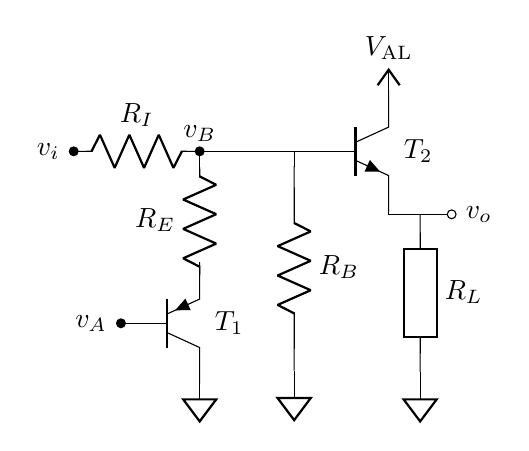
\begin{tikzpicture}[scale=0.8]
	% Paths, nodes and wires:
	\draw (3, 5) to[american resistor, l={$R_I$}, label distance=0.02cm] (5, 5);
	\draw node[npn] (N1) at (8, 5) {} node[anchor=west] at (N1.text){$T_2$};
	\draw[draw] (7.16, 5) -- (5, 5);
	\draw node[pnp] (N2) at (5, 2.27) {} node[anchor=west] at (N2.text){$T_1$};
	\draw (5, 3.02) to[american resistor, l={$R_E$}, label distance=0.02cm] (5, 4.75);
	\draw[draw] (4.16, 2.27) -- (3.75, 2.27);
	\draw (6.5, 4.77) to[american resistor, l={$R_B$}, label distance=0.02cm] (6.5, 1.52);
	\draw node[sground] at (5, 1.5) {};
	\draw node[sground] at (6.5, 1.52) {};
	\draw node[circ] (N3) at (3.75, 2.27) {} node[anchor=east] at (N3.west){$v_A$};
	\draw node[circ] (Vi) at (3, 5) {} node[anchor=east] at (Vi.west){$v_i$};
	\draw node[vcc] (N4) at (8, 5.77) {} node[anchor=south] at (N4.north){$V_\text{AL}$};
	\draw[draw] (5, 5) -| (5, 4.75);
	\draw[draw] (6.5, 4.75) -| (6.5, 5);
	\draw[draw] (8, 4.23) -| (8, 4) -- (9, 4);
	\draw node[ocirc] (Vo) at (9, 4) {} node[anchor=west] at (Vo.east){$v_o$};
	\draw (8.5, 4) to[european resistor, l={$R_L$}, label distance=0.02cm] (8.5, 1.5);
	\draw node[sground] at (8.5, 1.5) {};
	\draw node[circ] (Vb) at (5, 5) {} node[anchor=south] at (Vb.text){$v_B$};
\end{tikzpicture}
    \caption{Accent CV}
    \label{fig:accent-cv}
\end{figure}

Innanzitutto osserviamo che \(T_1\) non può entrare in saturazione perché \(\var{V}{CB,1} = -v_A \le \qty{0}{\volt}\), pertanto la giunzione collettore-base non può essere in conduzione.
Poiché la tensione in ingresso \(v_i\) è la tensione d'uscita del gate to trigger, per analizzare il funzionamento di questo circuito consideriamo due casi:

\begin{enumerate}
    \item Impulso, uscita del comparatore alta (\(v_i = +\var{V}{AL}\))
    \item Uscita del comparatore bassa (\(v_i = -\var{V}{AL}\))
\end{enumerate}

Nel primo caso ipotizziamo \(T_1\) e \(T_2\) in linearità, e verifichiamo che quest'ipotesi sia compatibile con i risultati.
Allora \(T_2\) è in configurazione di collettore comune e riporta, con un piccolo offset, la tensione che riceve sulla base (\(v_B\)).
Invece \(T_1\), siccome la giunzione emettitore-base è in conduzione, riporta \(v_A\) sul suo emettitore;
ai fini di questa analisi si comporta come un generatore di tensione di valore \(v_A + \var{V}{EB,1,on}\).
Ipotizzando che la corrente di base di \(T_2\) sia trascurabile, otteniamo per \(v_B\) la seguente espressione:
%
\begin{equation}
    v_B = \frac{R_I \parallel R_B}{R_E + R_I \parallel R_B} \left(v_A + \var{V}{EB,1,on} \right) +
    \frac{R_E \parallel R_B}{R_I + R_E \parallel R_B} \var{V}{AL}
\end{equation}
%
L'uscita del blocco è \(v_o = v_B - \var{V}{BE,2,on}\).

Nel secondo caso \(v_i = -\var{V}{AL}\) e risulta \(v_B < 0 \); entrambi i transistor sono in interdizione e l'uscita del blocco vale \(v_o = \qty{0}{\volt}\).

% TODO: inserire grafici dell'andamento di v_B

\subsection{T-Oscillator}
\subsubsection{Comportamento qualitativo nel dominio tempo}
\begin{figure}[ht]
    \centering
    \includegraphics[width=0.5\textwidth]{../images/Toscillator.png} 
    \label{fig:Toscillator}
\end{figure}

Il Toscillator è un circuito costituito da un solo amplificatore operazionale, due resistenze e due condensatori. Insieme formano un oscillatore a onda sinusoidale piuttosto strano che necessita di essere avviato con un impulso di tensione per iniziare a oscillare.
Tuttavia, anche quando avviato, non continuerà a oscillare come fanno gli altri oscillatori, ma l'ampiezza calerà rapidamente fino a scomparire del tutto. Questo comportamento non è ideale per la maggior parte degli scenari, ma è perfetto per il nostro.Vediamo come funziona.

\begin{figure}[ht]
    \centering
    \includegraphics[width=0.5\textwidth]{../images/Toscillator1.png} 
    \label{fig:Toscillator1}
\end{figure}

 Supponiamo che la tensione all'ingresso non invertente dell'opamp salti rapidamente da 0 a 1 volt. Per raggiungere uno stato di equilibrio, l'opamp cercherà di aumentare la tensione all'ingresso invertente fino a 1 volt anch'esso ( ricorda v+ = v- in un opamp).
 Per farlo, aumenterà inizialmente la sua tensione di uscita a 1 volt. Questo funzionerà all'inizio, poiché tale tensione attraversa direttamente i due condensatori e raggiunge così l'ingresso invertente.
 Tuttavia, a causa della presenza di una resistenza verso terra tra i due condensatori, vedremo una corrente che defluisce dal primo condensatore, il che significa che la tensione applicata al secondo condensatore, e successivamente all'ingresso invertente, diminuirà.

\begin{figure}[ht]
    \centering
    \includegraphics[width=0.5\textwidth]{../images/Toscillator2.png} 
    \label{fig:Toscillator2}
\end{figure}

Per compensare, l'op-amp aumenterà la sua tensione di uscita, ma facendo ciò, ancora più corrente verrà spremuta fuori dal primo condensatore, costringendo l'op-amp a spingere ancora di più.
Questo continuerebbe fino a quando l'op-amp raggiunge la tensione di alimentazione superiore, se non fosse per la resistenza di collegamento in retroazione.
Man mano che l'op-amp spinge sempre più forte, quella resistenza permette una piccola corrente di caricare il secondo condensatore dall'altro lato.
A un certo punto, questo processo aggiungerà più tensione sulla sinistra di quanta ne perderemo a destra, facendo sì che l'intero meccanismo si inverta.

\begin{figure}[ht]
    \centering
    \includegraphics[width=0.5\textwidth]{../images/Toscillator3.png} 
    \label{fig:Toscillator3}
\end{figure}


L'op-amp inizierà a ridurre la sua tensione di uscita per cercare di correggere, ma il problema è che ciò sottrarrà corrente dal primo condensatore e successivamente dal lato terra, aumentando la tensione tra i due condensatori e quindi all'ingresso invertente, il che costringerà l'op-amp a ridurre ulteriormente la sua tensione di uscita.
Alla fine raggiungeremo di nuovo un punto critico dove il meccanismo si invertirà, ma questa volta a una tensione di uscita leggermente inferiore.
Questo accade perché ad ogni ciclo di carica e scarica perdiamo un po' del momento iniziale. 

\begin{figure}[ht]
    \centering
    \includegraphics[width=0.5\textwidth]{../images/Toscillator4.png} 
    \label{fig:Toscillator4}
\end{figure}

Il circuito si comporta un po' come un pendolo, e quindi l'uscita prodotta è un'onda sinusoidale che oscilla attorno alla tensione dell'ingresso non invertente con un'ampiezza in continua diminuzione, che dovrebbe già suonare molto simile a un suono di grancassa se la frequenza è abbastanza bassa.
Per assicurarsi che lo sia, dobbiamo scegliere la giusta combinazione di valori per i condensatori e le resistenze.
Questo è un po' complicato, poiché tutti questi valori influenzano sia la frequenza che il decadimento contemporaneamente.
Nel circuito originale della grancassa dell'808, Roland utilizzava una resistenza di collegamento da 1 Megaohm, una resistenza verso terra da 51k e due condensatori da 15 nanofarad, ottenendo una frequenza di oscillazione di 50 hertz con un decadimento molto rapido.
Usiamo questi valori come punto di partenza. 

\subsubsection{Dominio frequenza}

Il circuito in retroazione puo' essere visto come un filtro elimina banda  (notch filter) 
che quando viene inserito nella retroazione di un amplificatore operazionale, trasforma il sistema in un filtro passa-banda. Utilizzando le equazioni per la rete a T di ponte, si possono trovare la frequenza centrale e il fattore di qualità del filtro in base ai valori combinati di resistenze e condensatori.

\begin{equation}
    f = \frac{1}{2 \pi\sqrt{R_1 R_2 C_1 C_2}}
\end{equation}

\begin{equation}
    Q = \frac{\sqrt{\frac{R_1}{R_2}}}{\sqrt{\frac{C_1}{C_2}} + {\frac{C_2}{C_1}}}
\end{equation}


Per utilizzare il filtro passa-banda come oscillatore, devono essere soddisfatte due condizioni: il cambiamento di fase intorno al loop dell'amplificatore operazionale deve essere un multiplo di 360 gradi (incluso 0 gradi) e ci deve essere un guadagno sufficiente.
Nel circuito del filtro a T di ponte, l'uscita dell'amplificatore operazionale ha uno sfasamento di 0 gradi alla frequenza centrale. Pertanto, se calcoliamo una frequenza centrale per una certa frequenza dell'oscillatore desiderata, possiamo scegliere i valori corretti dei componenti per ottenere quella frequenza centrale, che ci darà uno sfasamento di 0 gradi a quella frequenza. 

\begin{figure}[htp]
    \centering
    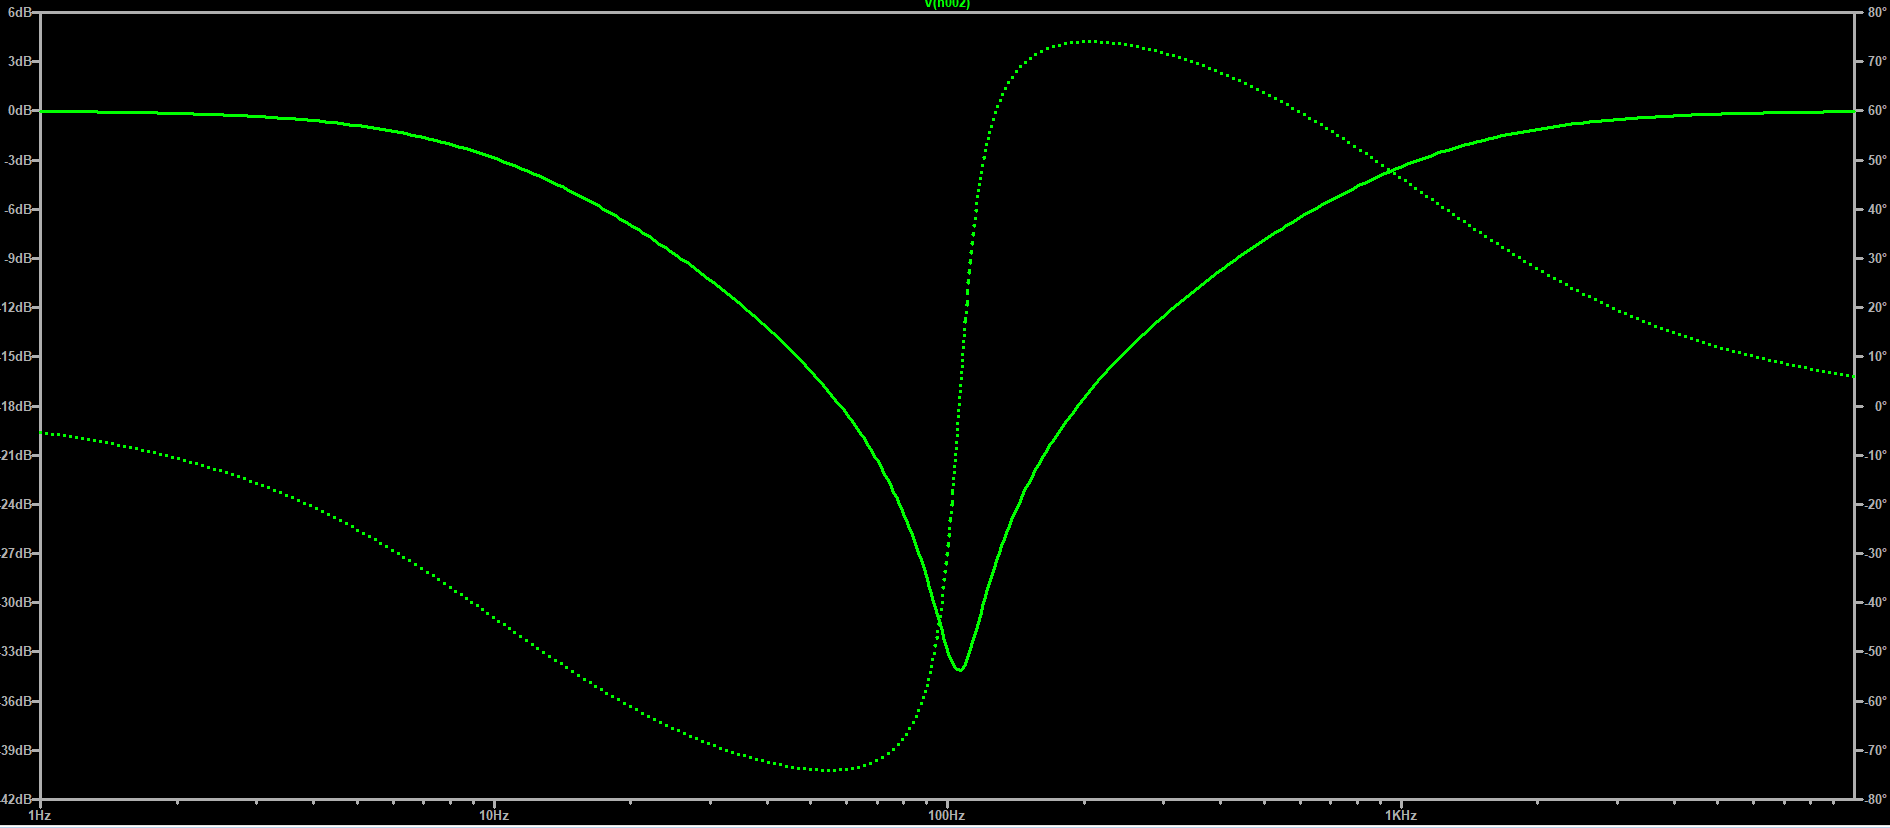
\includegraphics[width=\textwidth]{../images/notch2.png} 
    \caption{notch filter}
    \label{fig:Notch-filter}
\end{figure}

\begin{figure}[htp]
    \centering
    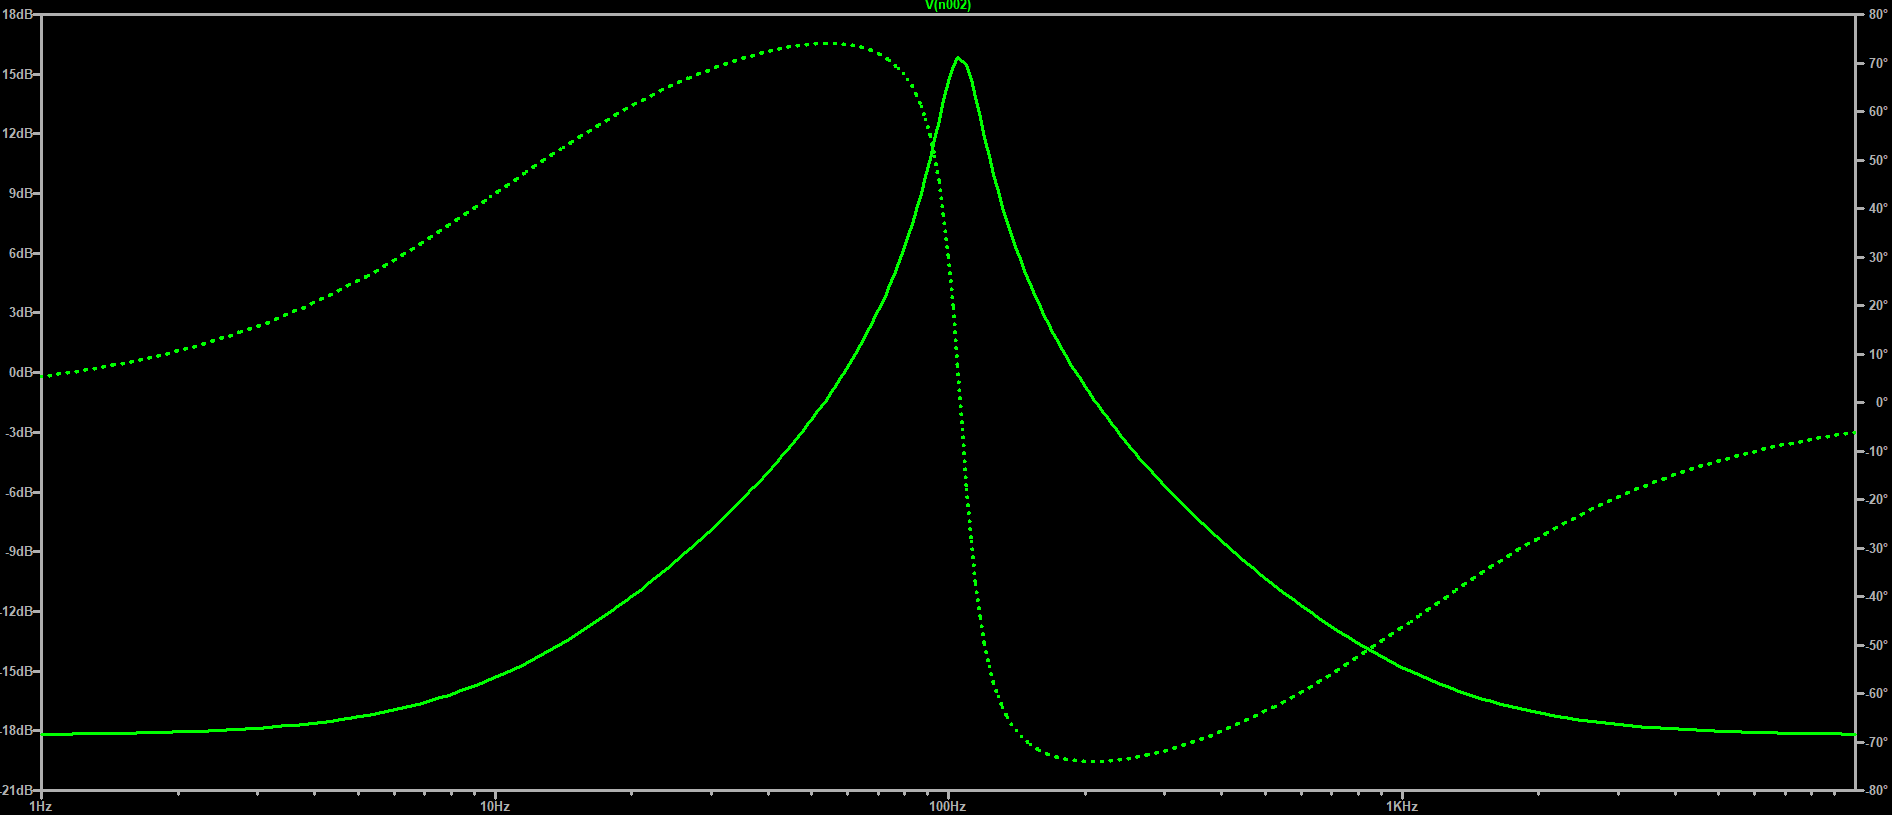
\includegraphics[width=\textwidth]{../images/toscillatorefrequency.png} 
    \caption{T-oscillator}
    \label{fig:Toscillator-plot}
\end{figure}

\end{document}

//Il blocco base consiste in un filtro passa alto e un comparatore (tensione soglia 3V). 
Quando applichiamo un onda quadra  il condensatore si carica fino a 5 V e poi tramite la resitenza al ground si scarica. La velocita' di scarica dipende dalla capacita del condensatore piu e' alta piu' tempo ci impiega. Quando la tensione sulla resitenza e' maggiore di quella del morsetto invertente 3V l'uscita dell'opamp va al max ovvero 12 V, mentre se minore a -12V (ricorda alimentazione).
Avendo bisogno di un impulso in uscita andiamo a prendere un condensatore con capacita piccola. Di conseguenza l'intervallo di tempo dove la tensione sulla resistenza e' maggiore di 3V sara' breve e quindi avremo in uscita un impulso.//